\section{Examples\label{sec:ch6:examples}}

Two different kinds of passive analog synthesis problems (frequency response matching and low-pass filter realizability)
have been chosen as the design examples. 
Both of these problem types have been studied previously, so we can readily make comparisons to previous results.
All runs were performed on a single computer with an i7-6800K at 3.8 GHz (up to 12 threads available), 32 GB DDR4 3200 MHz RAM, \textsc{Windows} 10 64-bit, and \textsc{Matlab} 2017a.
All aspects of the synthesis tool are coded in the \textsc{Matlab} language\footnote{The synthesis codes are available at Ref.~\cite{github-pm-circuits}.}.

\subsection{Frequency Response Matching\label{sec:ch6:freqresponse}}

\subsubsection{Synthesis Task}
The first example is based on Ref.~\cite{Grimbleby1995a}. Here we wish to synthesize circuits that match the following frequency response:
\begin{align}
\abs{F(j \omega)} = \sqrt{\frac{2 \pi}{10 \omega}}
\end{align}

\noindent over the frequency range:
\begin{align*}
0.2 \leq \frac{\omega}{2\pi} \leq 5
\end{align*}

\noindent with 500 logarithmically spaced evaluation points.
Since we have a desired magnitude response, not an explicit transfer function, traditional design methods cannot accommodate this synthesis task \cite{Grimbleby1995a}.

We will consider two sets of simple bounds on the coefficients of the resistors and capacitors:
\begin{align*}
\text{(set 1)} &\qquad \gls{resistance}\in[10^{-2}, 10^{0}]\ \Omega, \quad \gls{capacitance} \in [10^{-2}, 10^{0}] \text{ F} \\
\text{(set 2)} &\qquad R\in[10^{-2}, 10^{5}]\ \Omega, \quad C \in [10^{-10}, 10^{0}] \text{ F}
\end{align*}

\noindent and there are no additional general constraints.
The residual function is the pointwise decibel error in Eqn.~(\ref{eq:ch6:rk:1}).

\subsubsection{Circuit Structure Space\label{sec:ch6:mm:css}}

The desired circuit structure space is ``all topologies that have up to 6 impedance subcircuits and a required connection to the ground.''
Such a space is captured by:
\begin{subequations}
\label{eq:ch6:lib2}
\begin{align}
C &= \{ \xcolor{I}, \xcolor{O}, \xcolor{G}, \xcolor{Z}, \xcolor{N3}, \xcolor{N4}, \xcolor{N5}, \xcolor{N6}, \xcolor{N7}, \xcolor{N8}, \xcolor{N9} \} \\
P &=        \left[ 1\ 1\ 1\ 2\ 3\ 4\ 5\ 6\ 7\ 8\ 9 \right] \\
R_{\min} &= \left[ 1\ 1\ 1\ 1\ 0\ 0\ 0\ 0\ 0\ 0\ 0 \right] \\
R_{\max} &= \left[ 1\ 1\ 1\ 6\ 5\ 3\ 3\ 2\ 1\ 1\ 1 \right]
\end{align}
\end{subequations}

\noindent and includes all the NSCs from Sec.~\ref{sec:ch6:primitive}.
Only nine different orders of voltage nodes are used, as any higher-order nodes would not produce feasible topologies.
The specific values of $R_{\max}$ are the maximum number of replicates needed to still capture all possible feasible subcatalogs with respect to Eqn.~(\ref{eq:ch6:subcatalog:feas}).
The subcircuits for generating practical circuits will be series connections between $\{\xcolor{R}, \xcolor{C}\}$ components to replicate the elements available in Ref.~\cite{Grimbleby1995a}.
The primitive circuit library then has 393 unique graphs, and these graphs are expanded to 104,235 unique practical circuit graphs (see Table~\ref{tb:ch6:mm1:computational}).

\begin{table}[ht]
\centering
\caption{Computational cost of \nameref{sec:ch6:freqresponse} example.\label{tb:ch6:mm1:computational}}
\begin{tabular}{rrrr}
\hline \hline
                                    & Step                   & $t$ (s) & $N$ \\
\hline
\multirow{3}{*}{Circuit generation} & Primitive circuits     & 78 &  393 \\
                                    & Practical circuits     & 131  & 104,235  \\
                                    & Transfer functions     & 14,379  & 43,249   \\
 \arrayrulecolor{gray}\hline\arrayrulecolor{black}
 \multirow{2}{*}{Evaluation}        & Ref.~\cite{Grimbleby1995a}, set 1 & 29,303  & 43,249    \\
 & Ref.~\cite{Grimbleby1995a}, set 2 & 28,739  & 43,249    \\
\hline \hline
\end{tabular}
\end{table}

This synthesis task will utilize the template circuit in Fig.~\ref{fig:ch6:template:magnitude}.
Of the 104,235 practical circuit graphs, 43,249 were found to have unique transfer functions.
This difference is attributed to cases where two circuits that have the same transfer function but different colored graph representations.
For example, in some practical circuits, components do not show up in the transfer function (due to a functional short between the input and output nodes).
In these cases, the lower complexity circuit is always kept.
With the desired circuit library, we can now perform the sizing task to determine which circuits better satisfy the requirements of the synthesis task.

\subsubsection{Results}

\begin{figure*}[t]
\centering
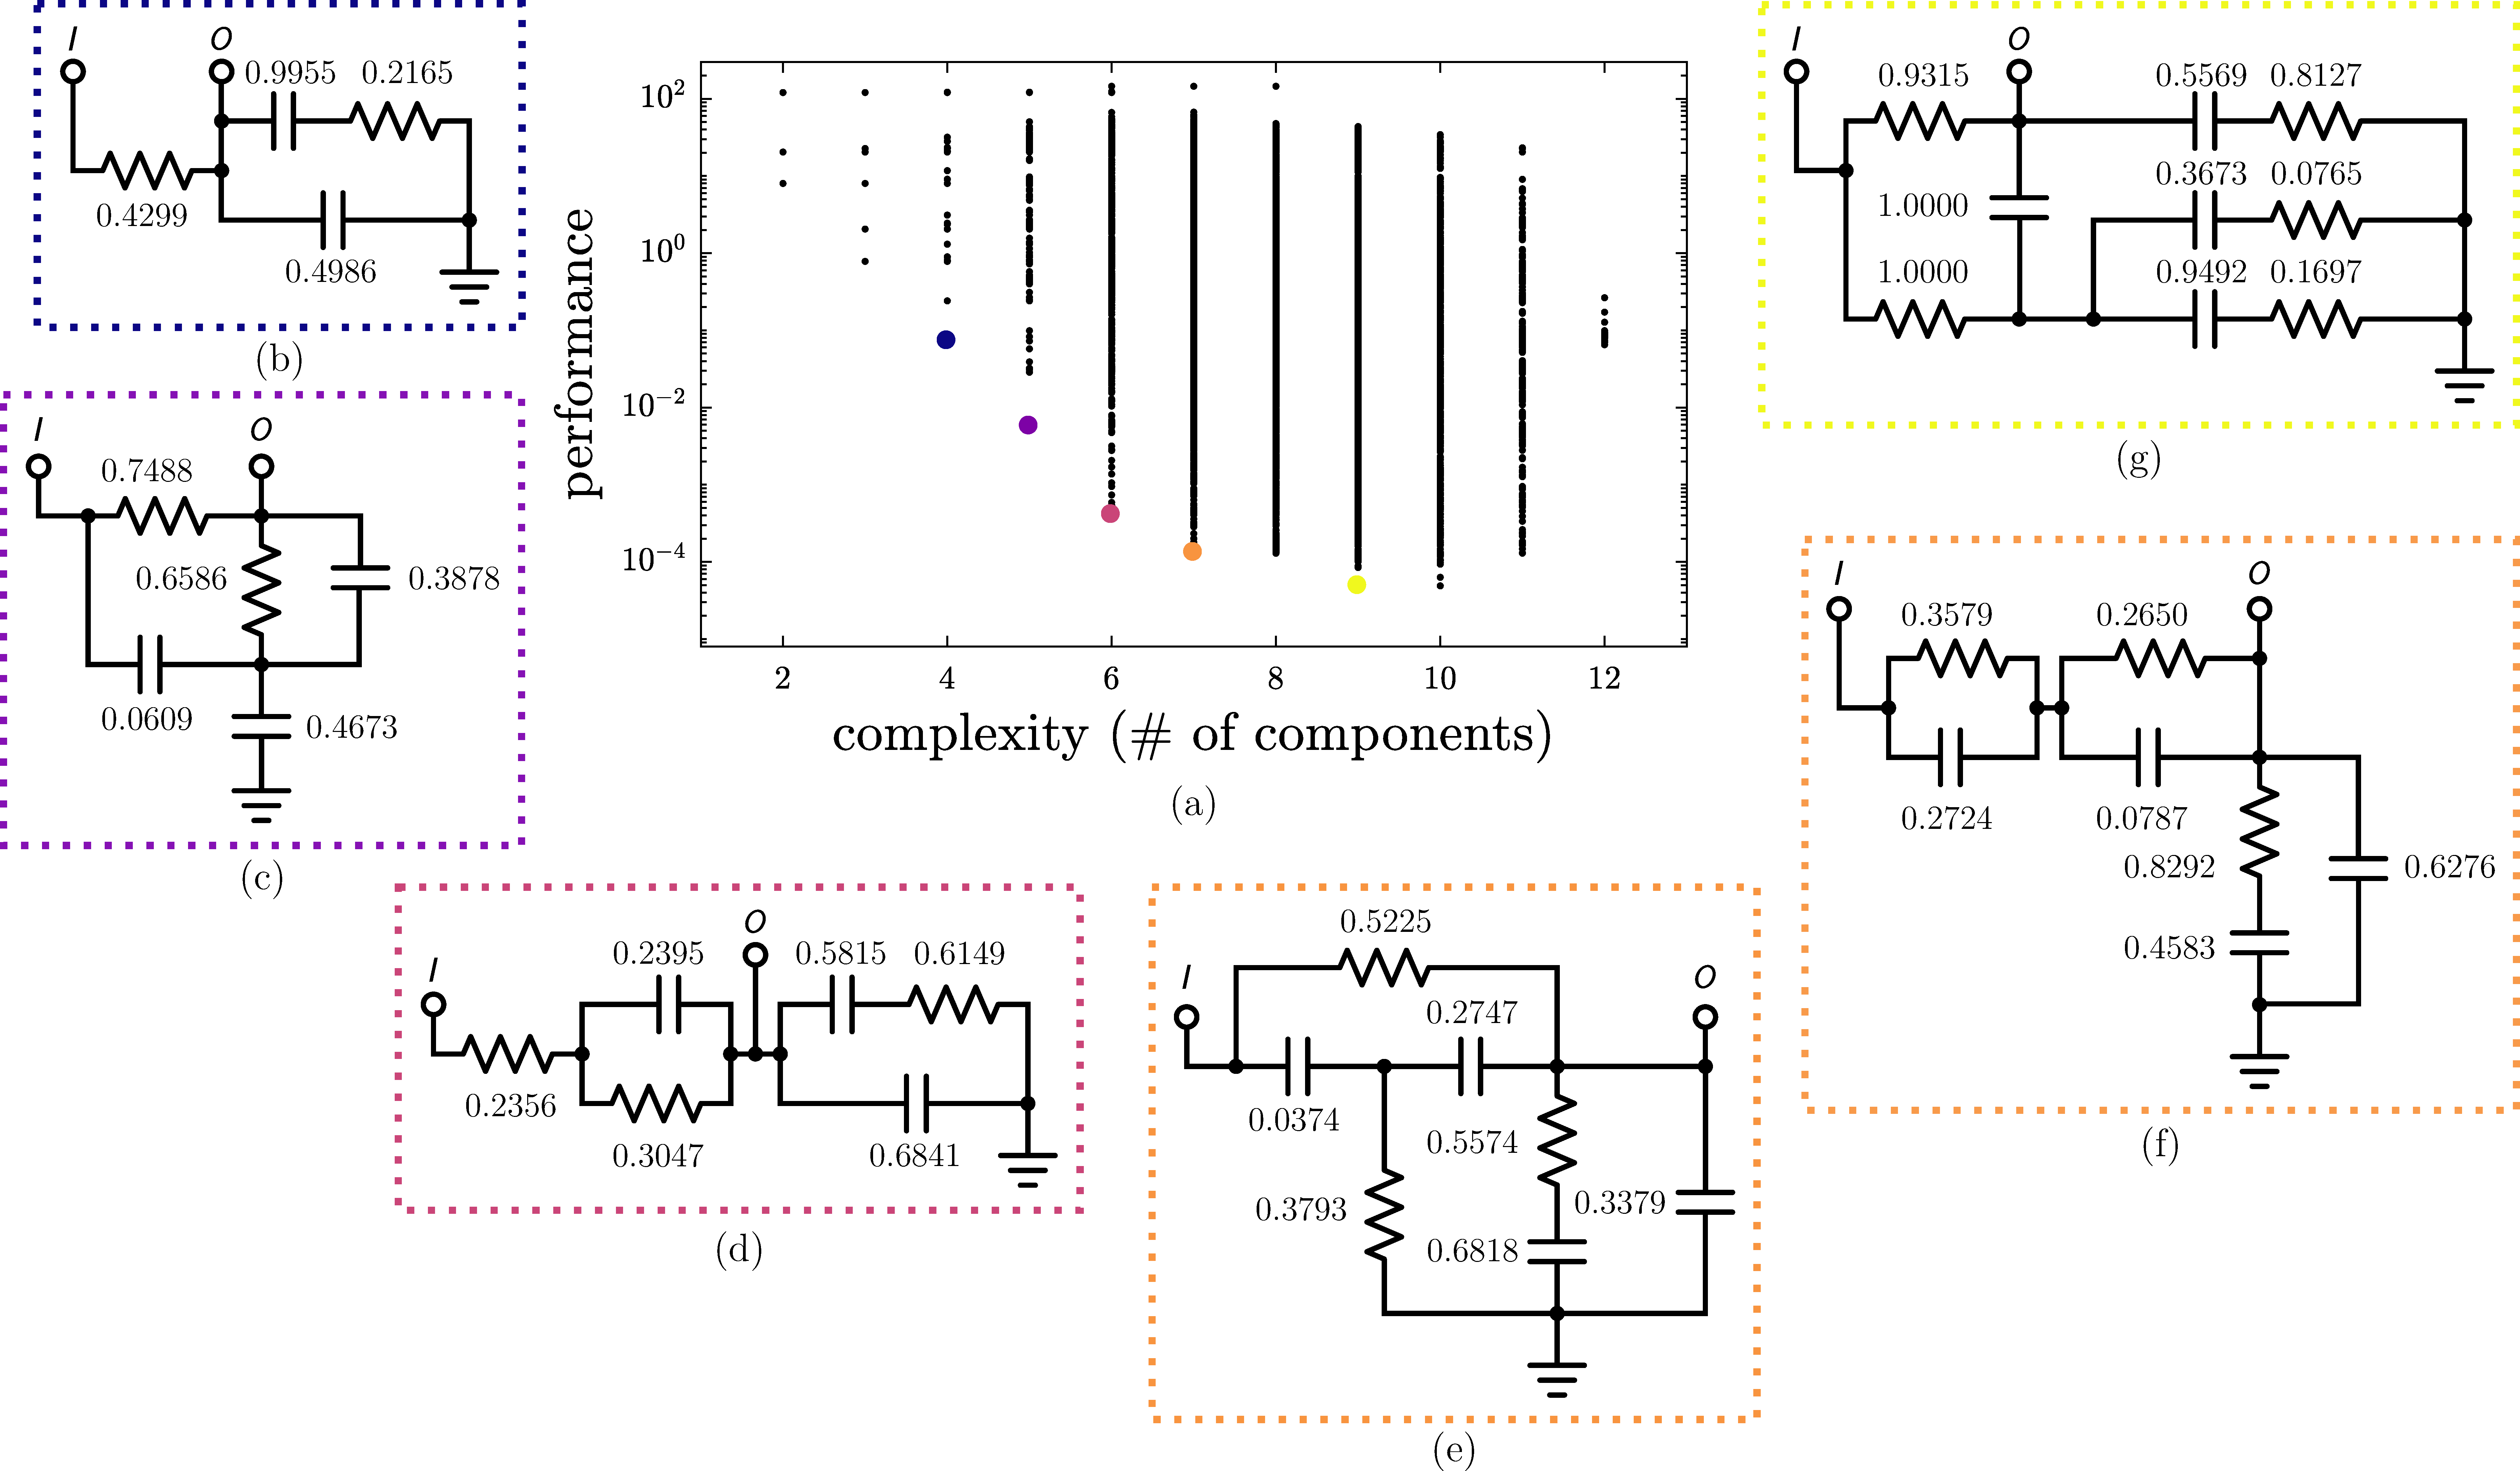
\includegraphics[width=\textwidth]{../ch6/figures/reduced/r_ex1_set1}
\caption[Performance vs. complexity for \nameref{sec:ch6:freqresponse} example using set 1 along with select Pareto optimal circuits.]{Performance vs. complexity (\# of components) for \nameref{sec:ch6:freqresponse} example using set 1 along with select Pareto optimal circuits (units are $\Omega$ and F).\label{fig:ch6:ex1:set1}}
\end{figure*}

The results for set 1 are summarized in Fig.~\ref{fig:ch6:ex1:set1}a where the performance for every circuit is shown, stratified by the complexity (or number of components).   
Select Pareto-optimal (performance cannot be improved without an increase in complexity) circuits are also shown in Figs.~\ref{fig:ch6:ex1:set1}a--g.
The desired magnitude response can be seen in Fig.~\ref{fig:mm1_magnitude} along with $\abs{G}$ for select circuits in Fig.~\ref{fig:ch6:ex1:set1}.

\begin{figure}
\centering
\begin{subfigure}[t]{0.5\textwidth}
\centering
% 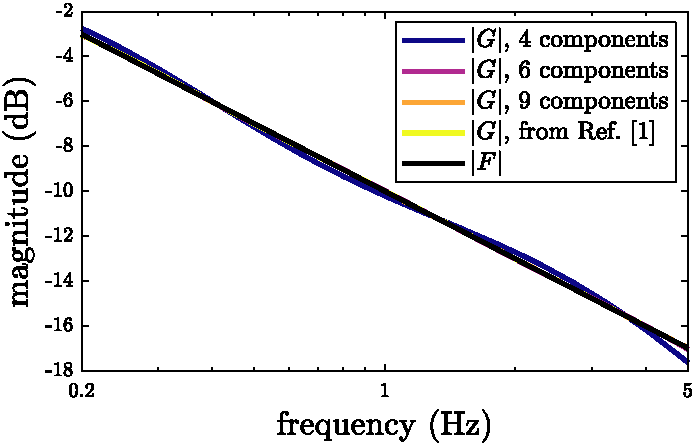
\includegraphics[width=\textwidth]{../ch6/figures/mm1_magnitude.pdf}
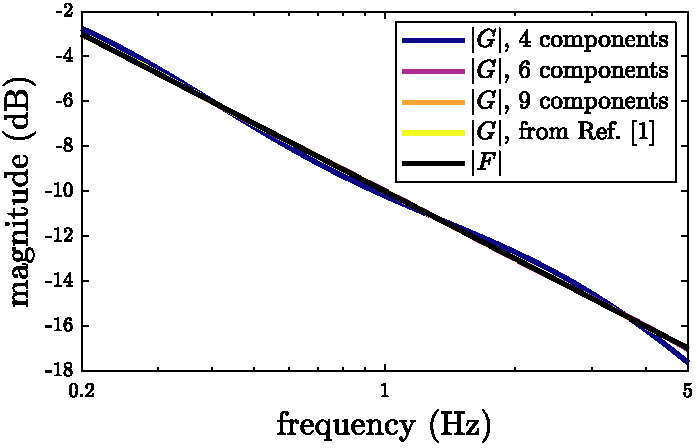
\includegraphics[width=\textwidth]{../ch6/figures/reduced/r_mm1_magnitude}
\caption{Both desired and circuit magnitude response.\label{fig:mm1_magnitude}}
\end{subfigure}%
\begin{subfigure}[t]{0.5\textwidth}
\centering
% 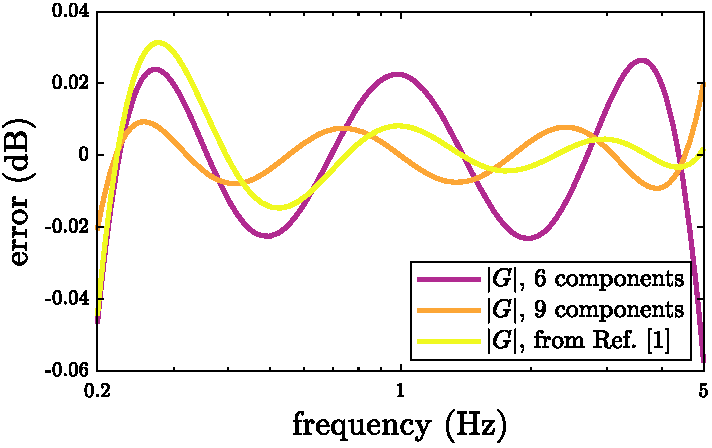
\includegraphics[width=\textwidth]{../ch6/figures/mm1_errors}
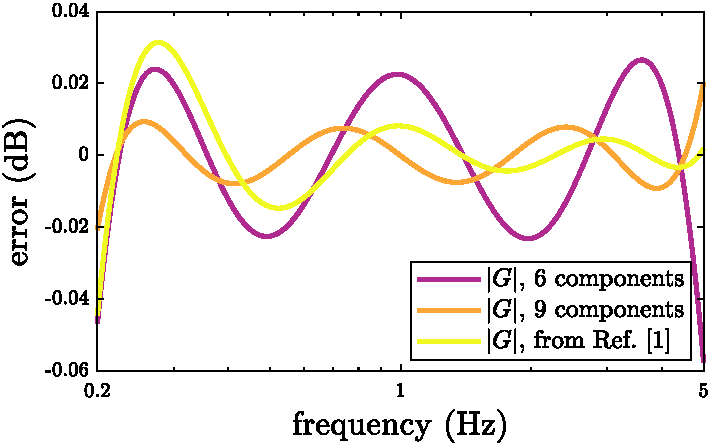
\includegraphics[width=\textwidth]{../ch6/figures/reduced/r_mm1_errors}
\caption{Errors.\label{fig:mm1_errors}}
\end{subfigure}%

\caption[Magnitude and errors over the desired frequency range using select circuits.]{Magnitude and errors over the desired frequency range using select circuits from Fig.~\ref{fig:ch6:ex1:set1}.\label{fig:mm1_magerrors}}

\end{figure}

% new paragraph
In fact, the included circuits are not unique Pareto-optimal circuits. 
For complexity levels of $\{4,5,6,7,9\}$, there are $\{5,22,57,200,2\}$ different circuits that produce the same level of performance.
This is due to each having nearly identical transfer functions using different circuit topologies.
For a specified number of poles and zeros, there is a lower bound on the performance (nonzero in this task) defined by a transfer function where the coefficients are tuned directly (sometimes called complex-curve fitting \cite{Levy1959a}).
Therefore, a set of circuits perform as well as possible under the pole/zero limitations defined by the circuit structure space and complexity level.
For example, consider the circuit in Fig.~\ref{fig:ch6:ex1:set1}b where $G$ contains 2 zeros and 3 poles, and produces a performance level of $7.3 \times 10^{-2}$. If we instead designed the polynomial coefficients directly, the lower bound on the performance is $2.9 \times 10^{-2}$; which is similar to the synthesized circuit but smaller.
See Table~\ref{tb:ch6:mm1:besttransfer} for this comparison at additional complexity levels and note the trend in the optimal orders of \gls{nz} and \gls{np}.

\begin{table}[ht]
\centering
\caption[Performance comparison between best and arbitrary circuit transfer functions.]{Performance level comparison between best circuit transfer function and best arbitrary transfer function for various complexity levels.\label{tb:ch6:mm1:besttransfer}}
\begin{tabular}{rrrrr}
\hline \hline
& & & \multicolumn{2}{c}{Performance} \\
$n_c$ & $n_z^{\glsfoo[noindex]{optimal}}$ & $n_p^*$ & Best circuit $G$ & Best $G$ \\
\hline
4 & 2 & 3 & $7.3\times10^{-2}$ & $2.9\times10^{-2}$ \\
5 & 3 & 3 & $5.7\times10^{-3}$ & $3.4\times10^{-3}$ \\
6 & 3 & 4 & $4.1\times10^{-4}$ & $4.0\times10^{-4}$ \\
7 & 4 & 4 & $1.3\times10^{-4}$ & $4.8\times10^{-5}$ \\
8 & 4 & 5 & $1.3\times10^{-4}$ & $5.6\times10^{-6}$ \\
9 & 5 & 5 & $4.8\times10^{-5}$ & $6.6\times10^{-7}$  \\
\hline \hline
\end{tabular}
\end{table}

% new paragraph
In a similar manner as set 1, the results for set 2 are summarized in
Fig.~\ref{fig:mm1_results_set2}.
In this set of results, an interesting pattern emerges, namely more discrete groupings of the performance levels and similarly valued groups are shared between different complexity levels.
With increased flexibility in the values of the passive component's coefficients, transfer functions with similar properties (e.g.,~the same order for $n_z$ and $n_p$) are attracted to similar performance levels during sizing.
This is further illustrated in Fig.~\ref{fig:mm1_cumpercent} where the performance is plotted by cumulative percentage of circuits that have at least the given performance level.
For set 1 we see little pattern in the performance curve but with set 2, we see more discrete performance levels.
In this figure we also see more circuits achieving a specified level of performance with the increased variable ranges in set 2 (i.e.,~the curve for set 2 is always below set 1).
In addition, many more circuits achieve the best performance level, but there is only a minor reduction of the objective compared to circuits sized using set 1.

\begin{figure}
\centering
% 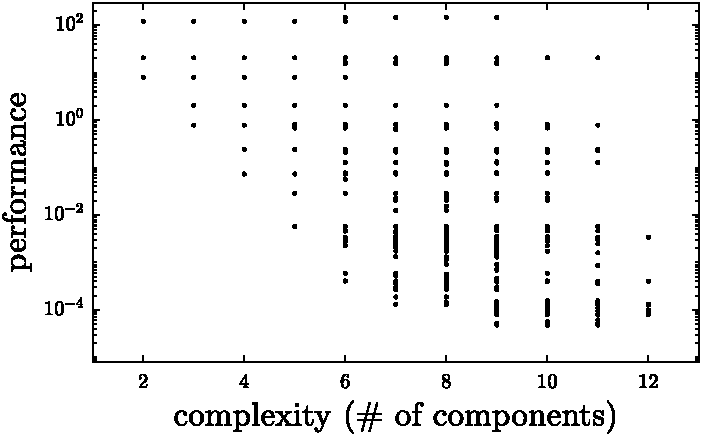
\includegraphics[width=0.9\columnwidth]{../ch6/figures/template1_lib5_CR_RESULTS_SET2}
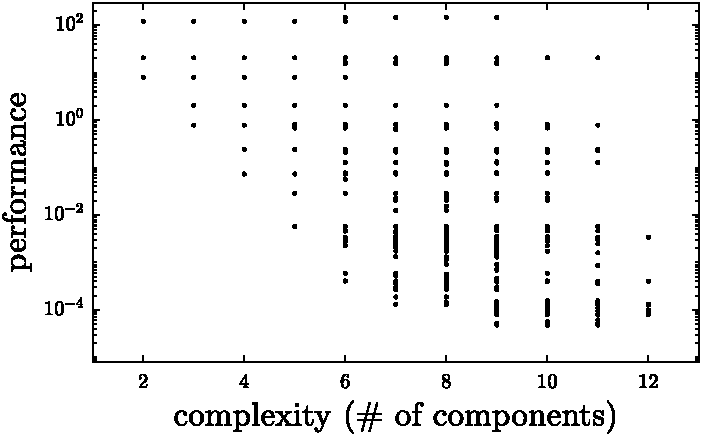
\includegraphics[width=0.5\textwidth]{../ch6/figures/reduced/r_template1_lib5_CR_RESULTS_SET2}
\caption[Performance vs. complexity for \nameref{sec:ch6:freqresponse} example using set 2.]{Performance vs. complexity (\# of components) for \nameref{sec:ch6:freqresponse} example using set 2.\label{fig:mm1_results_set2}}
\end{figure}

\begin{figure}[t]
\centering

\includegraphics[width=0.2\columnwidth]{../ch6/figures/template1_lib5_CR_RESULTS_Legend_FINAL.pdf}

\vspace{0.05in}

\begin{subfigure}[b]{0.3\columnwidth}
\centering
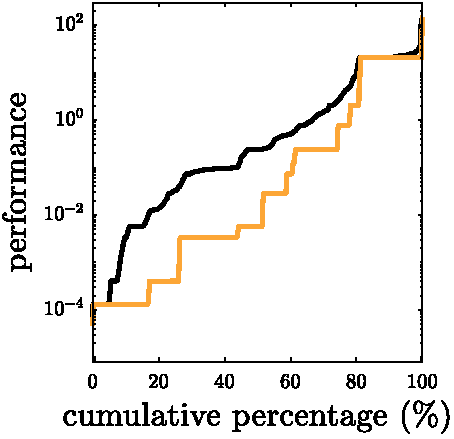
\includegraphics[width=\textwidth]{../ch6/figures/template1_lib5_CR_RESULTS}
\caption{All circuits.}
\end{subfigure}%
\begin{subfigure}[b]{0.3\columnwidth}
\centering
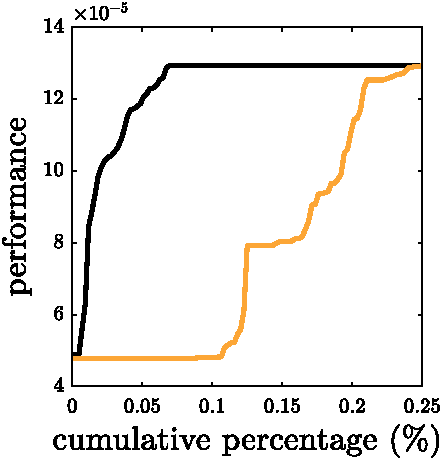
\includegraphics[width=\textwidth]{../ch6/figures/template1_lib5_CR_RESULTS_2}
\caption{Best circuits.}
\end{subfigure}%
\caption{Performance vs. cumulative percentage for \nameref{sec:ch6:freqresponse} example.\label{fig:mm1_cumpercent}}
\end{figure}

% new paragraph
A circuit of particular interest is the one found in Fig.~\ref{fig:ch6:ex1:set1}e, as it has the same topology as the circuit reported in Ref.~\cite{Grimbleby1995a}.
Since the topology and sizing tasks were performed simultaneously using an evolutionary approach in Ref.~\cite{Grimbleby1995a}, it could have been challenging to converge to the local optimum (something gradient-based methods do well).
However, it is extremely impressive that the synthesized circuit in Ref.~\cite{Grimbleby1995a} was close to the Pareto frontier (same topology, slightly worse performance level at $3.0 \times 10^{-4}$ with the error visualized in Fig.~\ref{fig:mm1_errors}).

% new paragraph
While the circuit in Fig.~\ref{fig:ch6:ex1:set1}g has the best performance level (under the enumerated circuit structure space), it would be up to the designer to decide if the increase in complexity is worth the performance improvement.
Having a large number of options provides the designer with additional flexibility when selecting a final circuit.

\subsection{Low-Pass Filter Realizability\label{sec:ch6:lpf}}

\subsubsection{Synthesis Task}

\begin{figure}
\centering
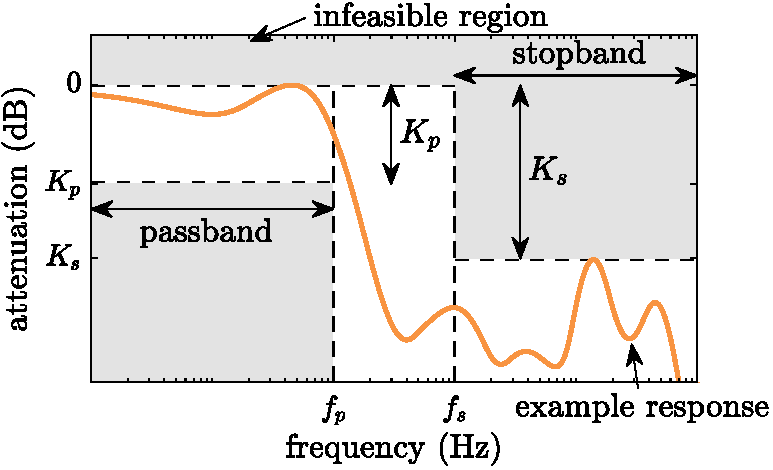
\includegraphics[width=0.6\textwidth]{../ch6/figures/reduced/r_filter_specs}
\caption{Low-pass filter specifications.\label{fig:ch6:filter:specs}}
\end{figure}

The second example is the synthesis of a \glsfirst{LPF}. A LPF attenuates signals above a certain frequency and passes all other signals.
The design specification of a LPF is shown in Fig.~\ref{fig:ch6:filter:specs}.
There are many classical synthesis methods for LPFs such as Butterworth, Chebyshev I, Chebyshev II, Elliptic,  Legendre-Papoulis, etc. \cite{Wanhammar2009a}.
LPFs are also frequently used as examples for evolutionary-based synthesis methods \cite{Das2007a, Gan2010a, Goh2001a, Grimbleby2000a, Koza1997a, Koza2000a, Lohn1999a}.
Here we will try to synthesize four LPFs with their specifications and variable bounds shown in Table~\ref{tb:ch6:lpfspecs}.

\subsubsection{Circuit Structure Space}

The desired circuit structure space is ``all topologies that have up to 7 passive components with an optional connection to the ground''.
Such a space is captured by:
\begin{subequations}
\label{eq:ch6:lib3}
\begin{align}
C &= \{ \xcolor{I}, \xcolor{O}, \xcolor{G}, \xcolor{Z}, \xcolor{N3}, \xcolor{N4}, \xcolor{N5}, \xcolor{N6}, \xcolor{N7}, \xcolor{N8}, \xcolor{N9} \} \\
P &=        \left[ 1\ 1\ 1\ 2\ 3\ 4\ 5\ 6\ 7\ 8\ 9 \right] \\
R_{\min} &= \left[ 1\ 1\ 0\ 1\ 0\ 0\ 0\ 0\ 0\ 0\ 0 \right] \\
R_{\max} &= \left[ 1\ 1\ 1\ 7\ 5\ 4\ 3\ 2\ 2\ 2\ 1 \right]
\end{align}
\end{subequations}

\noindent and includes all the NSCs from Sec.~\ref{sec:ch6:primitive}.
This is very similar to Eqn.~(\ref{eq:ch6:lib2}), except $\xcolor{Z}$ now has up to seven replicates, $\xcolor{G}$ is optional, and some of the $\xcolor{N}x$ maximum replicate numbers have changed based on what is needed for Eqn.~(\ref{eq:ch6:subcatalog:feas}).
The subcircuits for generating practical circuits will be series connections between $\{\xcolor{L},\xcolor{C}\}$ components to replicate the elements typically used in LPFs.
The primitive circuit library then has 5,300 unique graphs and these graphs are expanded to 1,804,496 unique practical circuit graphs (see Table~\ref{tb:ch6:lpf:computational}).

\begin{table}[ht]
\centering
\caption{Computational cost of \nameref{sec:ch6:lpf} example.\label{tb:ch6:lpf:computational}}
\begin{tabular}{rrrr}
\hline \hline
 & Step                   & $t$ (s) & $N$ \\
\hline
\multirow{3}{*}{Circuit generation} & Primitive circuits  & 2,694 & 5,300  \\
 & Practical circuits & 6,330  & 1,804,496  \\
 & Transfer functions & 20,460 & 123,156   \\
 \arrayrulecolor{gray}\hline\arrayrulecolor{black}
 \multirow{4}{*}{Evaluation}        & Task \#1 & 235,810 & 123,156     \\
 & Task \#2 & 80,788 &  38,172   \\
 & Task \#3 & 83,231 & 38,172    \\
 & Task \#4 & 606 & 281    \\
\hline \hline
\end{tabular}
\end{table}

This synthesis task will utilize the template circuit in Fig.~\ref{fig:ch6:template:filter} with parameters $\{\gls{vs},\gls{Rs},R_l\}$ valued at $\{2 \text{V}, 1 \text{k}\Omega, 1 \text{k}\Omega\}$.
Of the 1,804,496 practical circuit graphs, 123,156 were found to have less than 7 components and remain unique transfer functions.
The practical circuit graph representation can be used directly to count the number of components before the transfer function is constructed.

\subsubsection{Results}

\begin{table}[ht]
\centering
%--------------------------------
\begin{subfigure}[t]{\textwidth}
\centering
\begin{tabular}{cccccccc}
\hline \hline
\# & c.f. & \gls{fp} (Hz) & \gls{fs} (Hz) & \gls{Kp} (dB) & \gls{Ks} (dB) & \gls{inductance} bounds (H) & $C$ bounds (F) \\
\hline
1 & \cite{Lohn1999a, Goh2001a} & 925 & 3200 & 3.01 & 22.0 & $\left[0.1\text{m}, 1.5\right]$ & $\left[0.1\text{p}, 200\mu\right]$ \\ % (6)
2 & \cite{Gan2010a} & 1000 & 2000 & 1.00 & 60.0 & $\left[0.01\text{m}, 10\right]$ &$ \left[0.1\text{p}, 100\mu\right]$ \\ % (11) 
3 & \cite{Das2007a} & 800 & 2000 & 0.60 & 68.0 & $\left[0.1\text{m}, 1\right]$ & $\left[100\text{p}, 1\mu\right]$ \\ % ()
4 & \cite{Lohn1999a, Goh2001a} & 1000 & 2000 & 0.01 & 63.5 & $\left[0.1\text{m}, 1.5\right]$ & $\left[0.1\text{p}, 200\mu\right]$ \\
\hline \hline
\end{tabular}
\caption{Specifications.}
\end{subfigure}
%--------------------------------
\begin{subfigure}[t]{\textwidth}
\centering
\begin{tabular}{cccc}
\hline \hline
\# & \# feasible & \% feasible & $\min n_c$ \\
\hline
1 & 38172 & 30.99 & 3   \\ % (6)
2 & 280 & 0.23 & 6 \\ % (11) 
3 & 197 & 0.16 & 6 \\ % ()
4 & 0 & 0 & $>7$ \\
\hline \hline
\end{tabular}
\caption{Results.}
\end{subfigure}

\caption[\nameref{sec:ch6:lpf} specifications and results.]{Summary of \nameref{sec:ch6:lpf} specifications and results.\label{tb:ch6:lpfspecs}}

%--------------------------------
\end{table}

The results for this example are summarized in Table~\ref{tb:ch6:lpfspecs} with the number of synthesized feasible circuits, the percentage of circuit topologies that were feasible after sizing, and the minimum number of components needed to satisfy the synthesis specifications.
The tasks had increasingly more difficult to satisfy specifications.

% study 1
\begin{figure}
\centering

\begin{subfigure}[t]{0.16\textwidth}
\centering
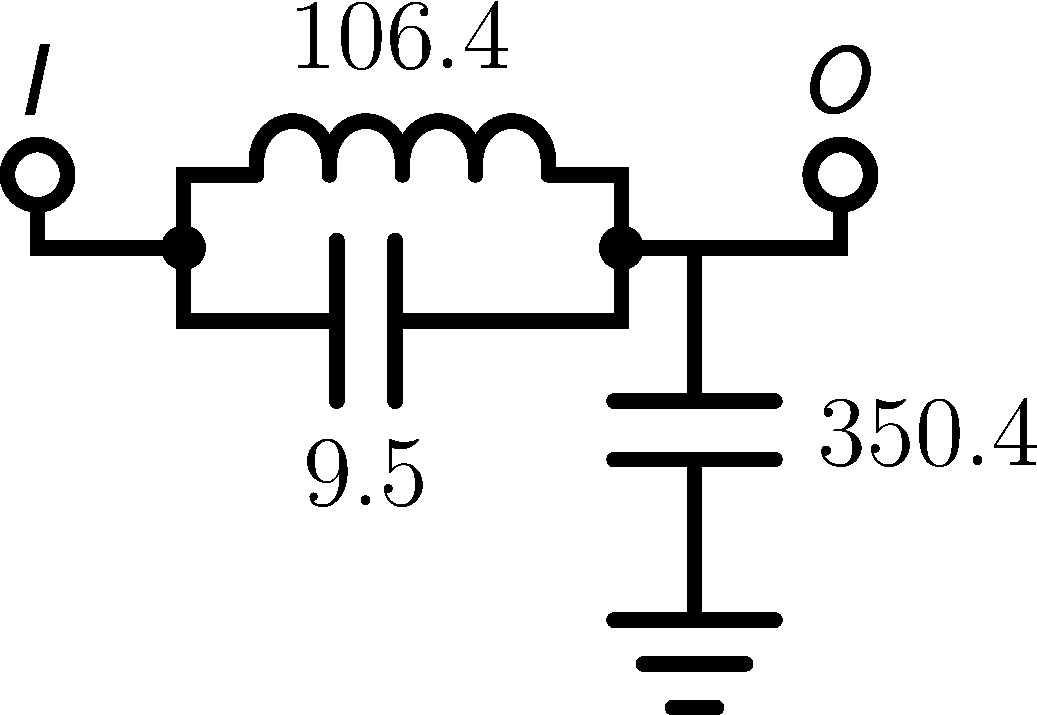
\includegraphics[scale = 0.14]{../ch6/figures/lpf1_circuit1}
\caption{\label{fig:lpf1_circuita}}
\end{subfigure}%
\begin{subfigure}[t]{0.16\textwidth}
\centering
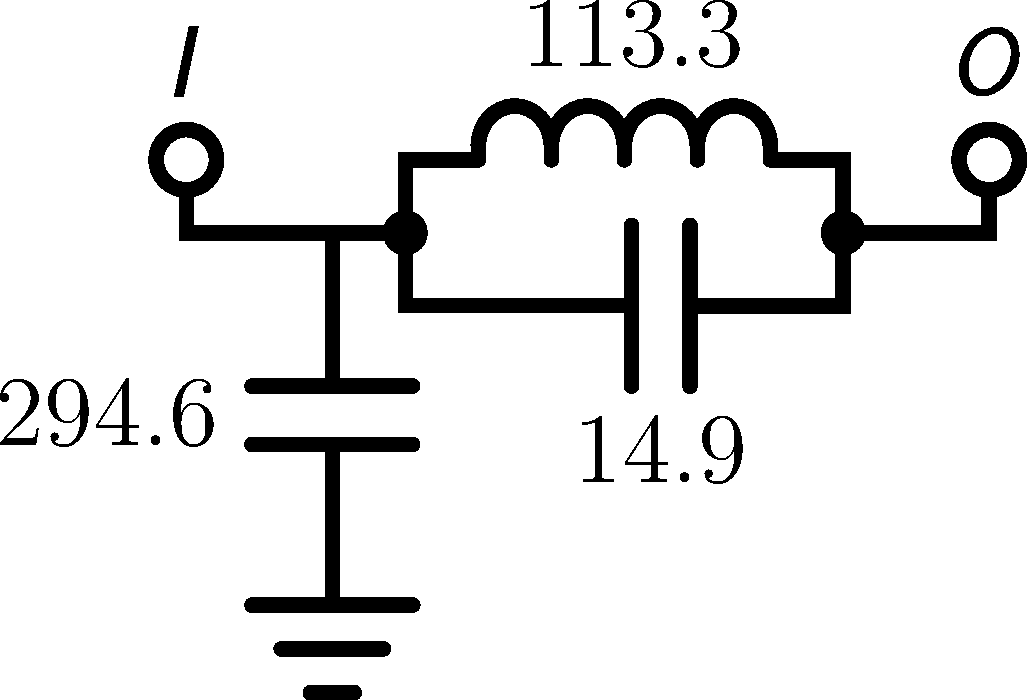
\includegraphics[scale = 0.14]{../ch6/figures/lpf1_circuit2}
\caption{\label{fig:lpf1_circuitb}}
\end{subfigure}%
\begin{subfigure}[t]{0.16\textwidth}
\centering
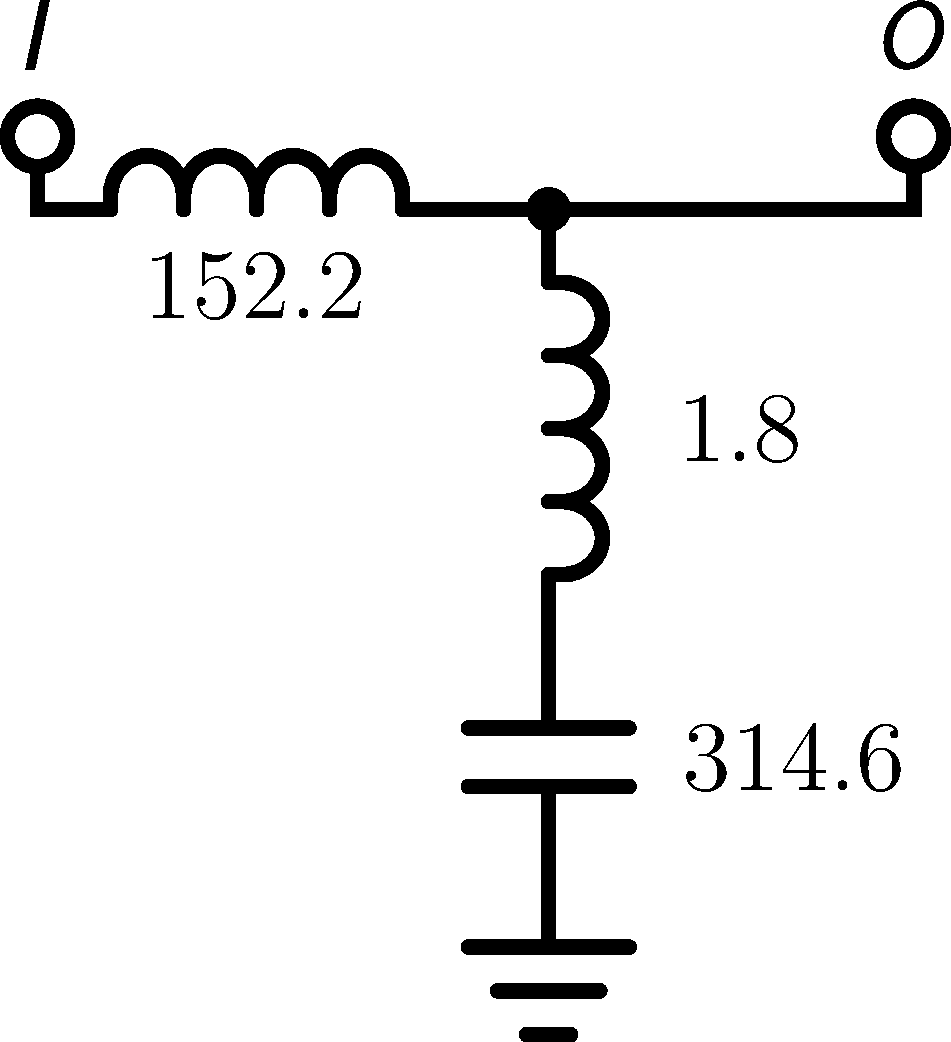
\includegraphics[scale = 0.14]{../ch6/figures/lpf1_circuit4}
\caption{\label{fig:lpf1_circuitc}}
\end{subfigure}%
\begin{subfigure}[t]{0.16\textwidth}
\centering
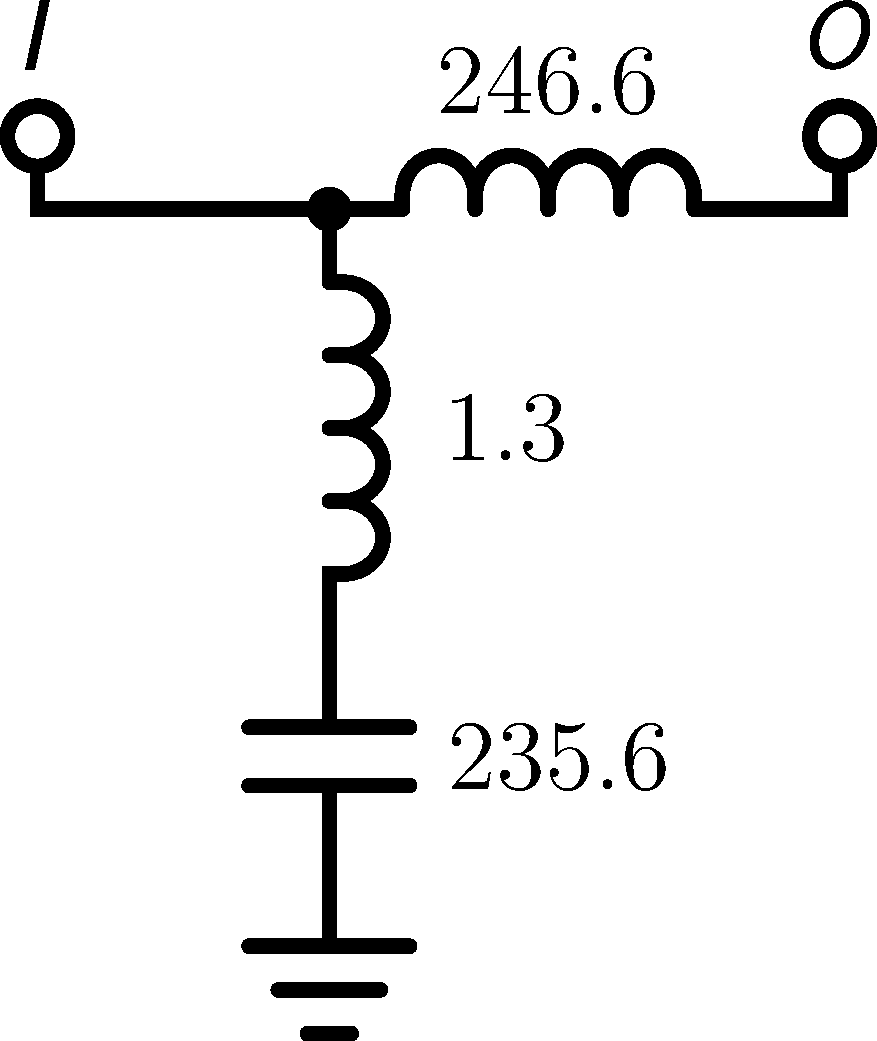
\includegraphics[scale = 0.14]{../ch6/figures/lpf1_circuit5}
\caption{\label{fig:lpf1_circuitd}}
\end{subfigure}%
\begin{subfigure}[t]{0.16\textwidth}
\centering
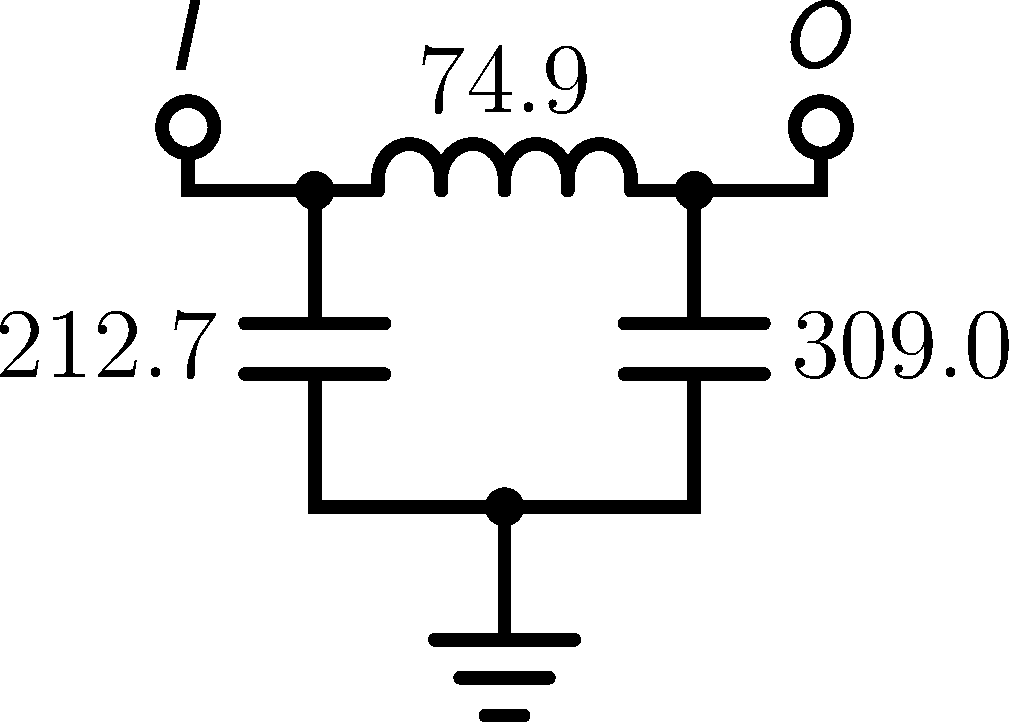
\includegraphics[scale = 0.14]{../ch6/figures/lpf1_circuit3}
\caption{\label{fig:lpf1_circuite}}
\end{subfigure}%
\begin{subfigure}[t]{0.16\textwidth}
\centering
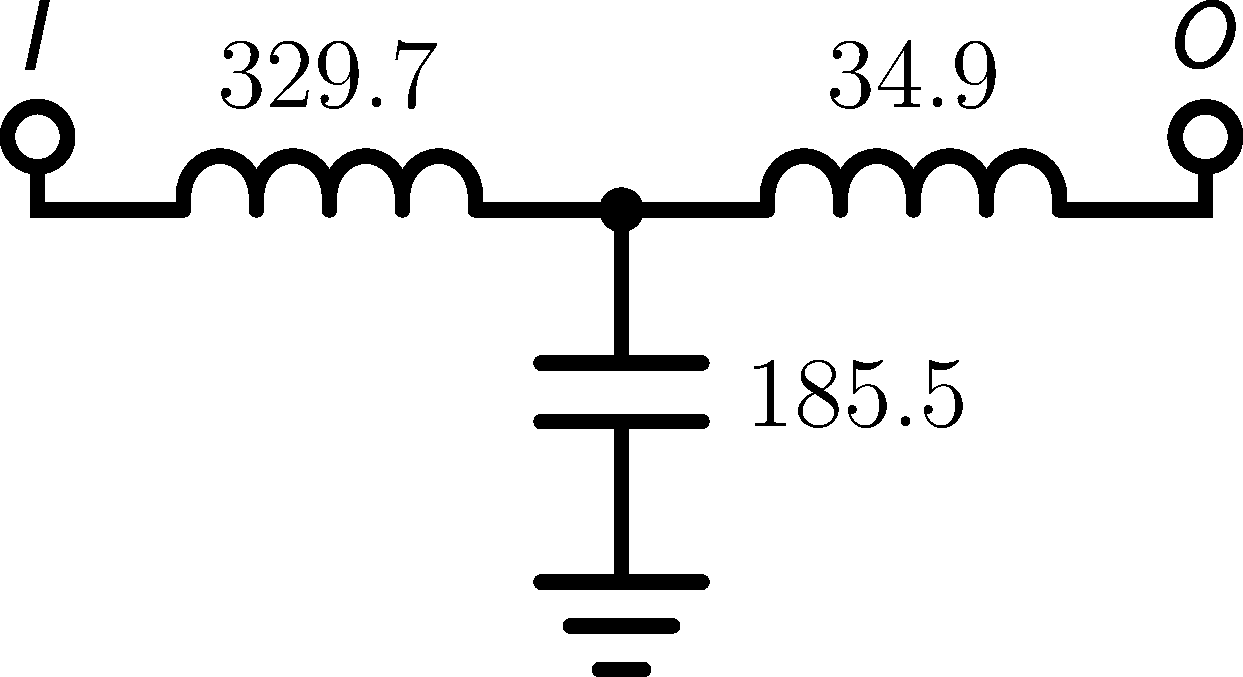
\includegraphics[scale = 0.14]{../ch6/figures/lpf1_circuit6}
\caption{\label{fig:lpf1_circuitf}}
\end{subfigure}%
\vspace{0.06in}
\begin{subfigure}[t]{\textwidth}
\centering
% 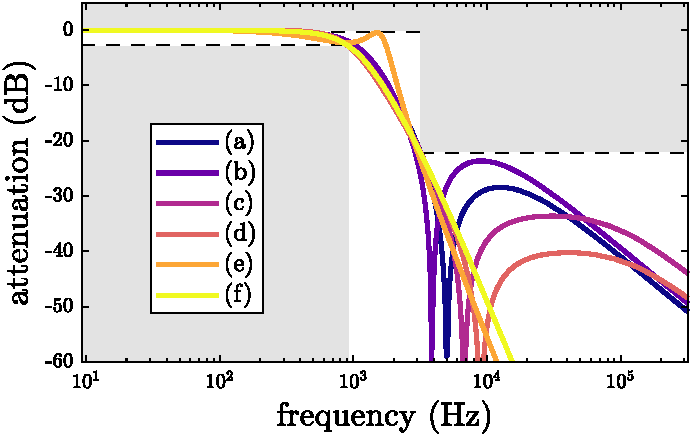
\includegraphics[width=\textwidth]{../ch6/figures/lpf1_magnitude}
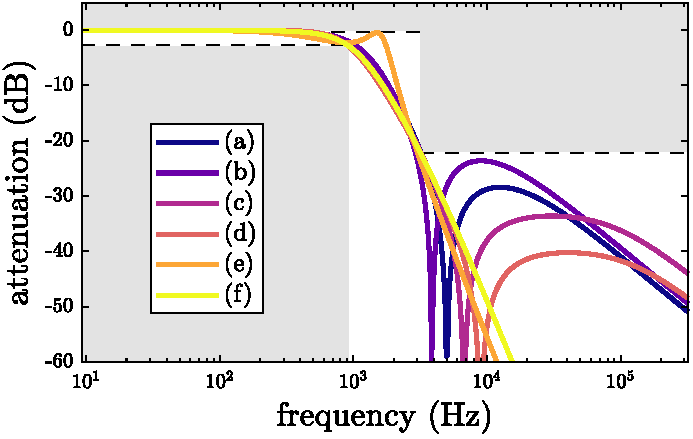
\includegraphics[width=0.5\textwidth]{../ch6/figures/reduced/r_lpf1_magnitude}
\caption{\label{fig:lpf1_magnitude}}
\end{subfigure}%

\caption[All feasible, minimum complexity circuits and attenuation responses for \nameref{sec:ch6:lpf} task \#1.]{All feasible, minimum complexity circuits and attenuation responses for \nameref{sec:ch6:lpf} task \#1 (units are mH and nF).\label{fig:lpf1}}

\end{figure}

The first study is based on examples in Refs.~\cite{Lohn1999a, Goh2001a}, and the specifications were chosen such that they could be satisfied using a third-order Butterworth filter \cite{Lohn1999a}.
This implies that there should be at least one three-component topology that satisfies the specifications (ignoring the variable bounds).
In fact, there are six different three-component topologies that satisfy the requirements, all shown in Figs.~\ref{fig:lpf1_circuita}--\ref{fig:lpf1_circuitf}.
The circuits in Fig.~\ref{fig:lpf1_circuita} and Fig.~\ref{fig:lpf1_circuitb} are topologically similar to one another, as well as Fig.~\ref{fig:lpf1_circuitc} and Fig.~\ref{fig:lpf1_circuitd}.
The other two are well known topologies; Fig.~\ref{fig:lpf1_circuite} is a $\pi$-section, and Fig.~\ref{fig:lpf1_circuitf} is a T-section.
Their attenuation responses are shown in Fig.~\ref{fig:lpf1_magnitude}; all responses are within the specifications.

% new paragraph
The best circuit for task \#1 found in Ref.~\cite{Goh2001a} is Fig.~\ref{fig:lpf1_circuitb}; thus, their evolutionary approach did find one of the minimum-complexity circuits. 
The best circuit from Ref.~\cite{Lohn1999a} had seven components; it is not reported as it is not a minimum-complexity topology.
Since enumeration was used, we can look at the likelihood that certain topologies would have been feasible.
For topologies with up to seven components, 30.99\% of the topologies are feasible (see Table~\ref{tb:ch6:nc:feasible:task1} for the percentage for each complexity level).

\begin{table}
\centering
\caption{Task \#1 feasible vs. total number of circuits for different complexity levels.\label{tb:ch6:nc:feasible:task1}}
\begin{tabular}{rrrr}
\hline \hline
& \multicolumn{2}{c}{Circuits} & \\
$n_c$ & Feasible & Total & \%  \\
\hline
1 & 0 & 2 & 0.0 \\
2 & 0 & 12 & 0.0 \\
3 & 6 & 60 & 10.0 \\
4 & 62 & 338 & 18.3 \\
5 & 534 & 2,192 & 24.4 \\
6 & 4,240 & 14,685 & 28.9 \\
7 & 33,330 & 105,867 & 31.5 \\
\hline \hline
\end{tabular}
\end{table}

% study 2
\begin{figure}
\centering
\begin{subfigure}[t]{0.25\textwidth}
\centering
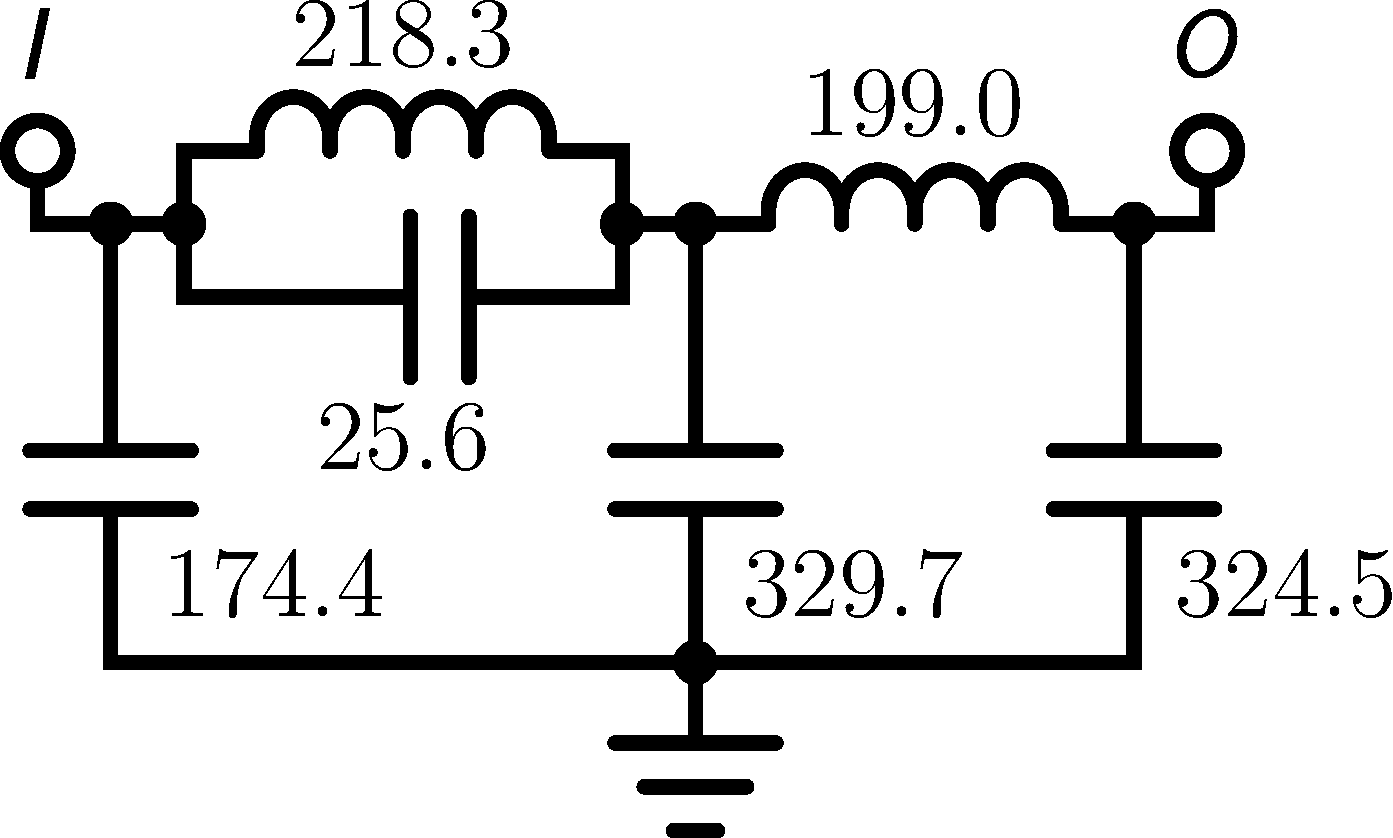
\includegraphics[scale = 0.14]{../ch6/figures/lpf2_circuit1}
\caption{\label{fig:lpf2_circuita}}
\end{subfigure}%
\begin{subfigure}[t]{0.25\textwidth}
\centering
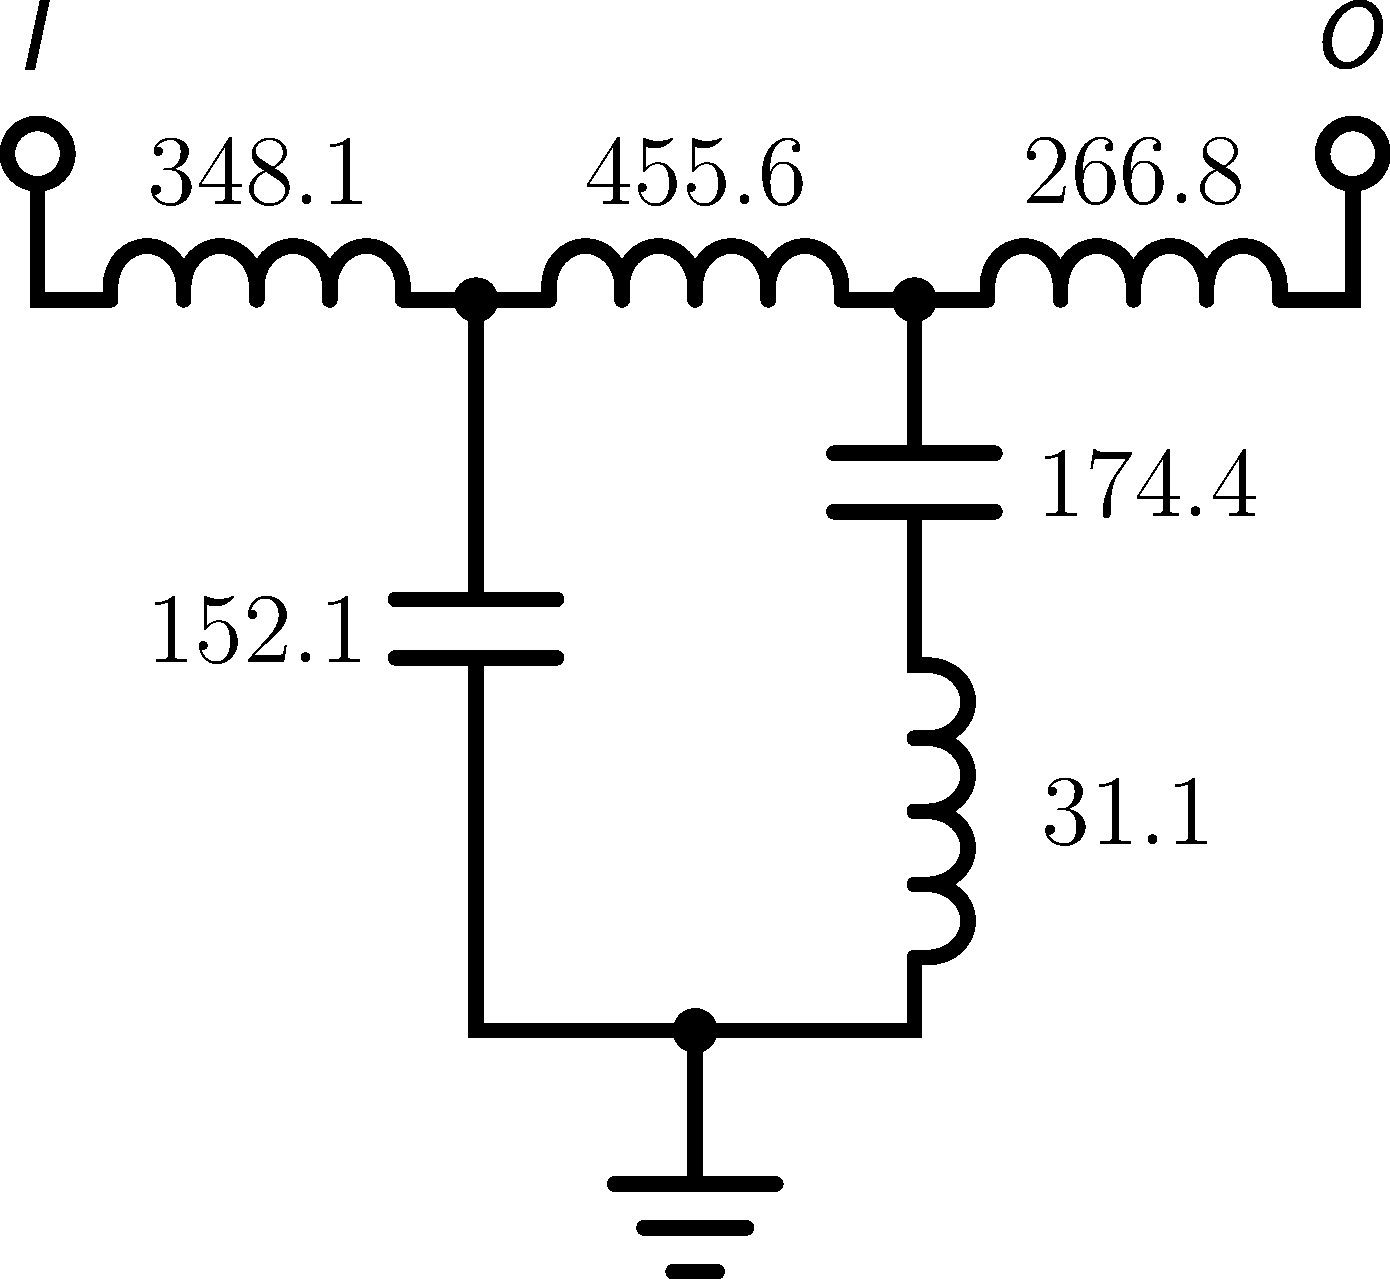
\includegraphics[scale = 0.14]{../ch6/figures/lpf2_circuit2}
\caption{\label{fig:lpf2_circuitb}}
\end{subfigure}%
% \vspace{0.06in}
\begin{subfigure}[t]{0.5\textwidth}
\centering
% 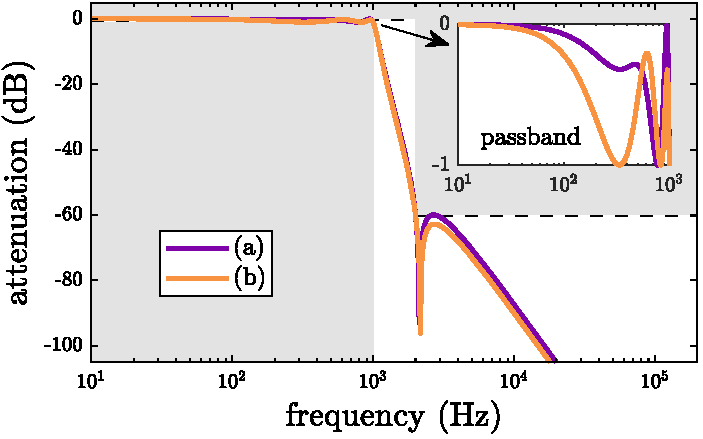
\includegraphics[width=\textwidth]{../ch6/figures/lpf2_magnitude}
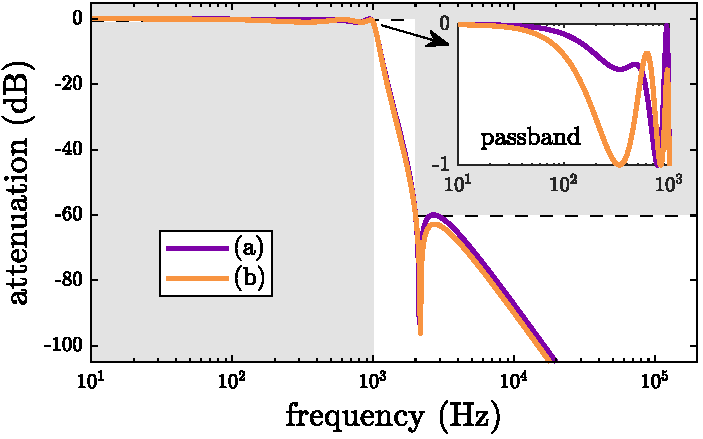
\includegraphics[width=\textwidth]{../ch6/figures/reduced/r_lpf2_magnitude}
\caption{\label{fig:lpf2_magnitude}}
\end{subfigure}%

\caption[Select feasible, minimum complexity circuits and attenuation responses for \nameref{sec:ch6:lpf} task \#2.]{Select feasible, minimum complexity circuits and attenuation responses for \nameref{sec:ch6:lpf} task \#2 (units are mH and nF).\label{fig:lpf2}}

\end{figure}

The specifications for task \#2 are more stringent.
Because of this, we can take the 38,204 feasible circuits from task \#1 as the starting set of circuits since any circuit that is not feasible in task \#1 will not be feasible in task \#2.
From this, only 280 circuits are found to be feasible with the minimum $n_c$ being six components.
Two of the eleven minimum-complexity circuits are shown in Figs.~\ref{fig:lpf2_circuita}--\ref{fig:lpf3_circuitb}.
Their attenuation responses are shown in Fig.~\ref{fig:lpf2_magnitude} (note the magnified region to highlight constraint satisfaction in the passband).

In Ref.~\cite{Gan2010a}, the reported circuit had eight components.
A direct comparison is not a fair assessment, as their study limited the preferred (discrete) component values (E12 series).
However, we can see that Fig.~\ref{fig:lpf2_circuita} is the same as their reported topology when \textsf{C4} and \textsf{C5} are removed.
An alternative complexity metric is the number of inductors as inductors can be bulky, heavy, and expensive compared to capacitors \cite{Wanhammar2009a}.
Under this metric, Fig.~\ref{fig:lpf2_circuita} is the minimum inductor solution (with two alternatives).
A similar discussion can be had with the task \#1 results, where only one inductor is needed in three of the circuits, such as in Fig.~\ref{fig:lpf1_circuita}.

% study 3
\begin{figure}
\centering
\begin{subfigure}[t]{0.25\textwidth}
\centering
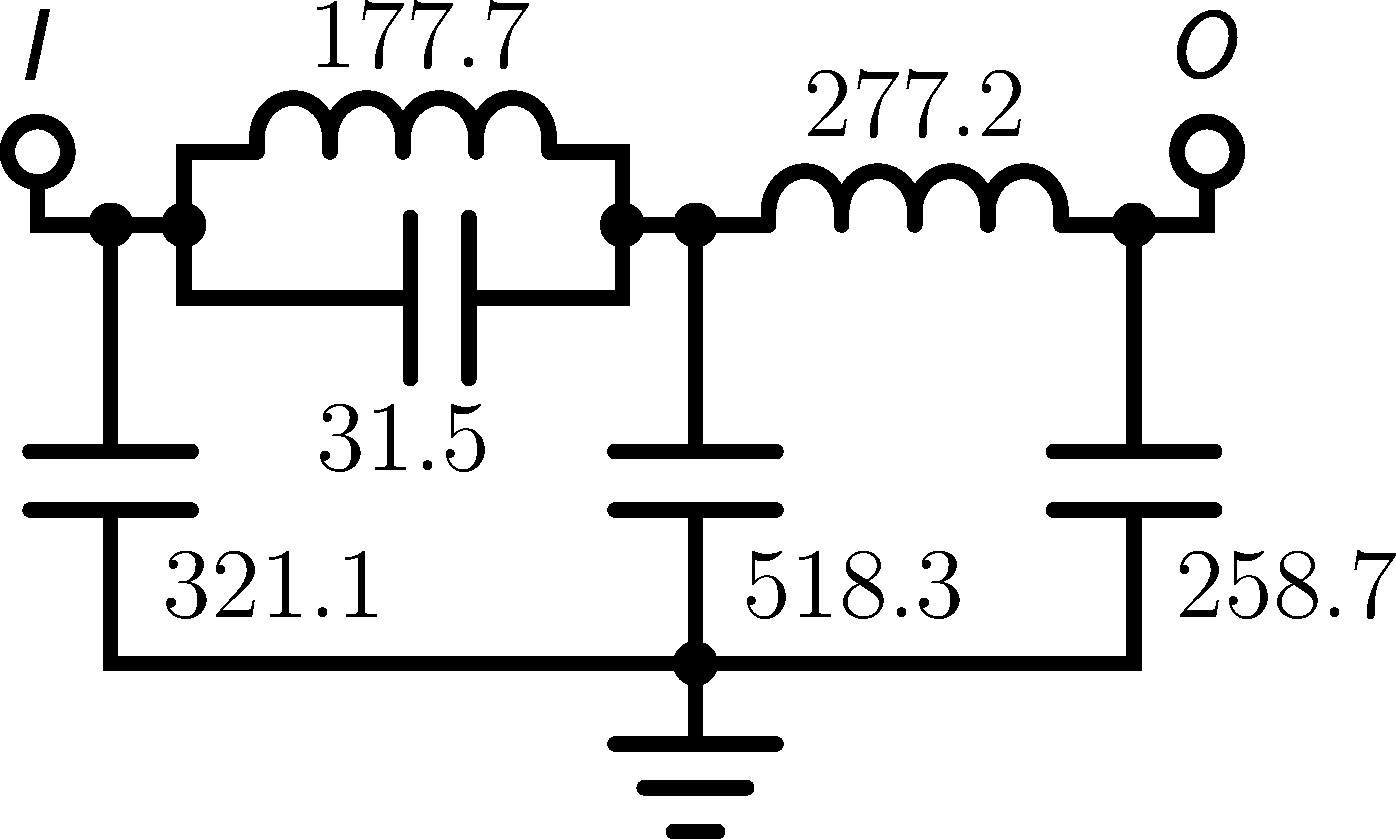
\includegraphics[scale = 0.14]{../ch6/figures/lpf3_circuit1}
\caption{\label{fig:lpf3_circuita}}
\end{subfigure}%
\begin{subfigure}[t]{0.25\textwidth}
\centering
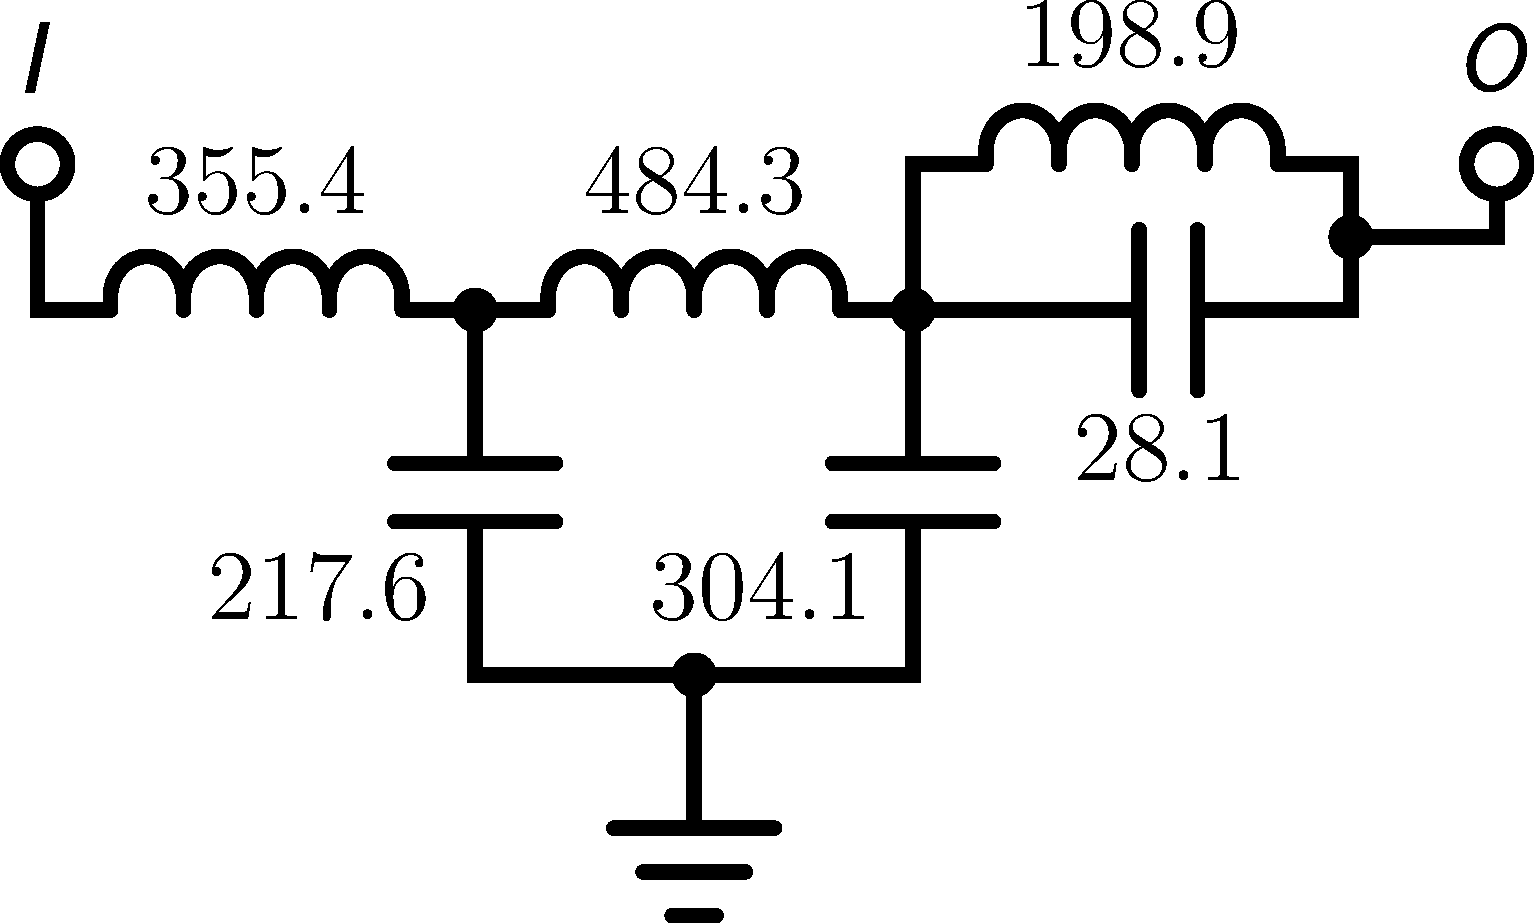
\includegraphics[scale = 0.14]{../ch6/figures/lpf3_circuit2}
\caption{\label{fig:lpf3_circuitb}}
\end{subfigure}%
\begin{subfigure}[t]{0.25\textwidth}
\centering
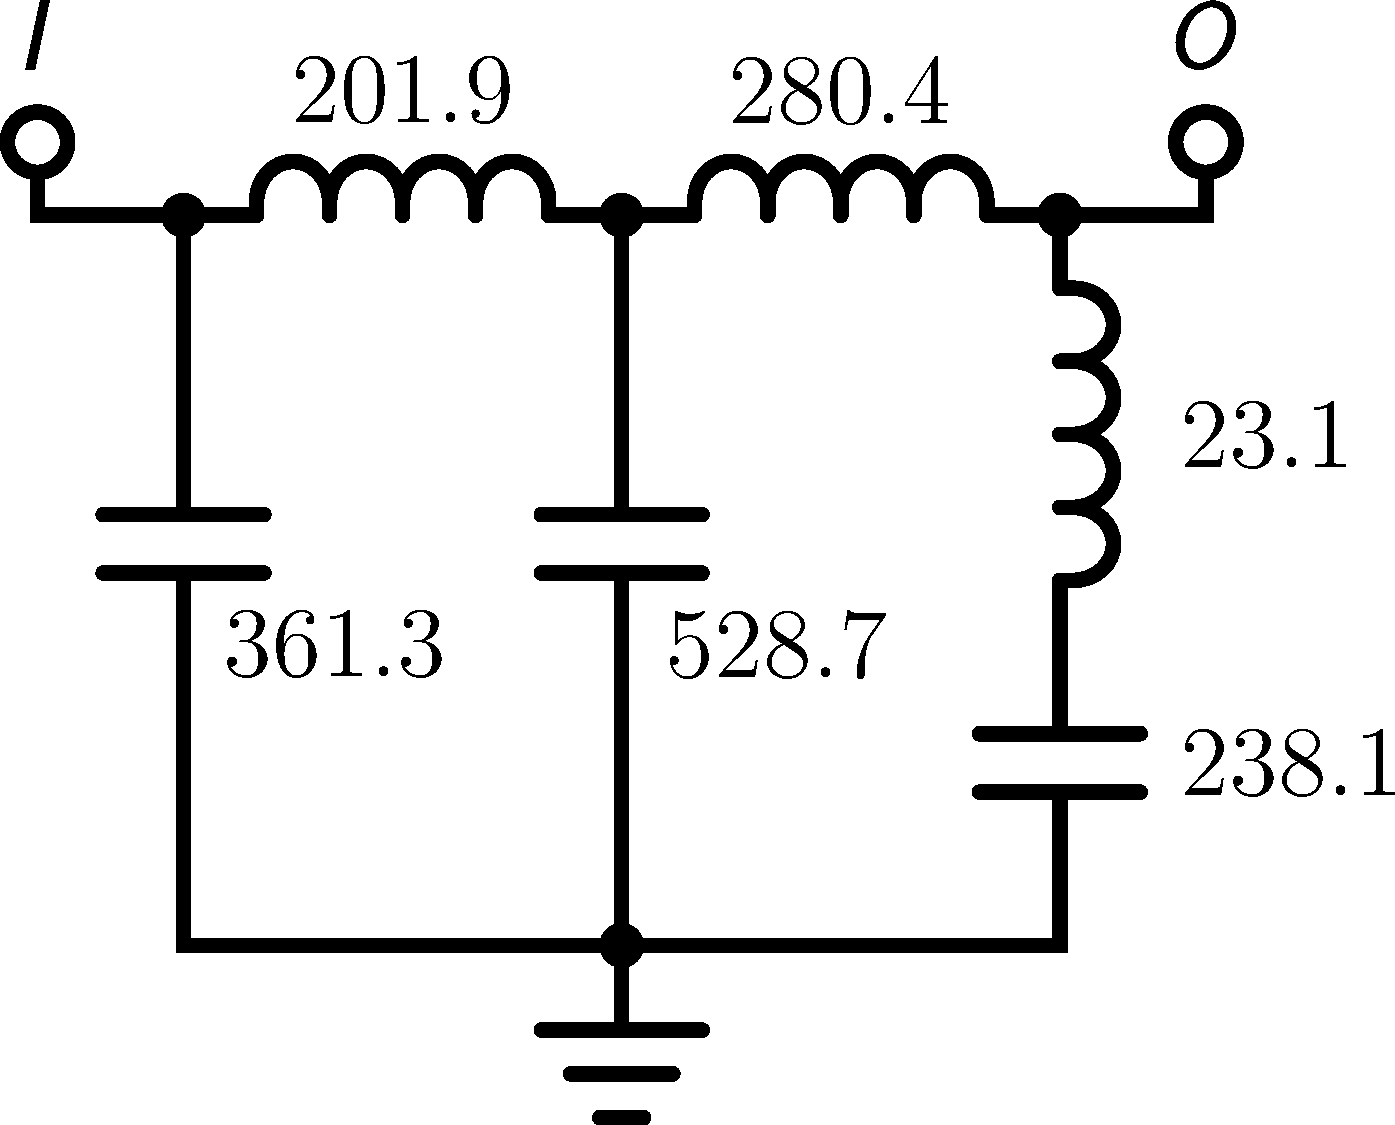
\includegraphics[scale = 0.14]{../ch6/figures/lpf3_circuit3}
\caption{\label{fig:lpf3_circuitc}}
\end{subfigure}%
\begin{subfigure}[t]{0.25\textwidth}
\centering
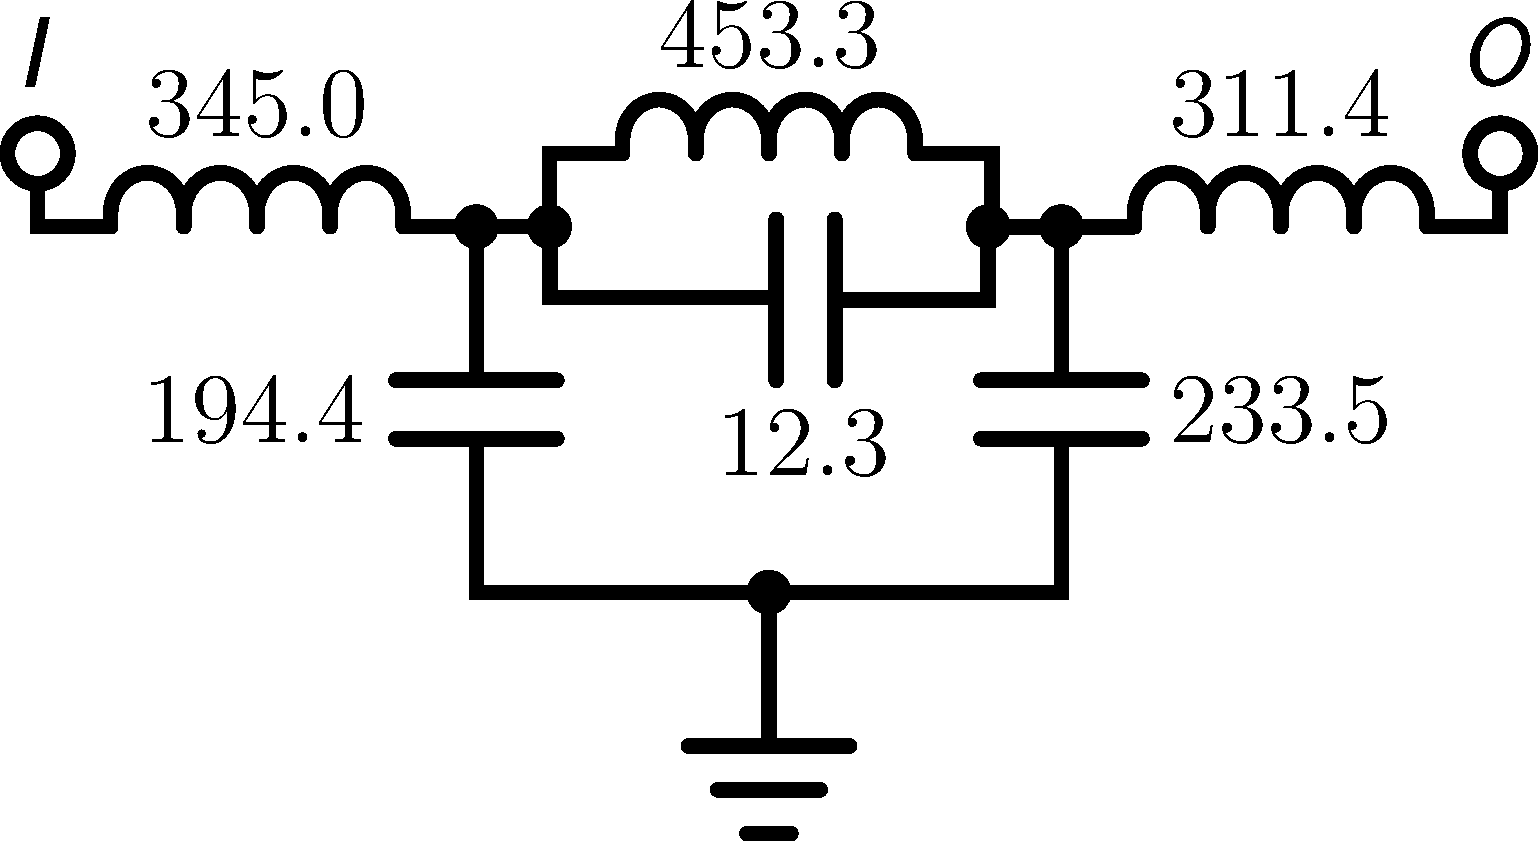
\includegraphics[scale = 0.14]{../ch6/figures/lpf3_circuit4}
\caption{\label{fig:lpf3_circuitd}}
\end{subfigure}%
\vspace{0.06in}
\begin{subfigure}[t]{\textwidth}
\centering
% 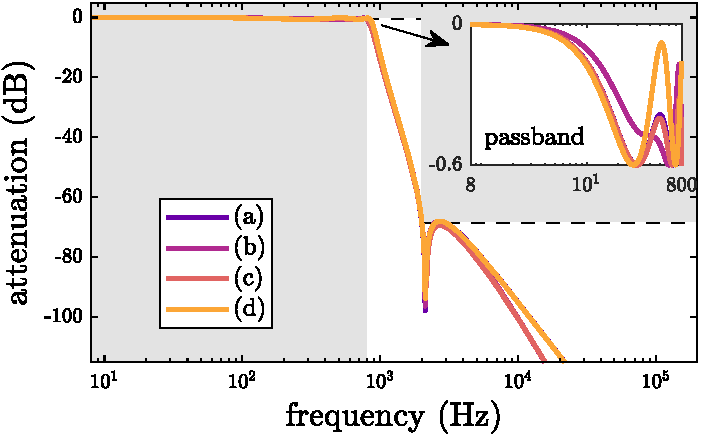
\includegraphics[width=\textwidth]{../ch6/figures/lpf3_magnitude}
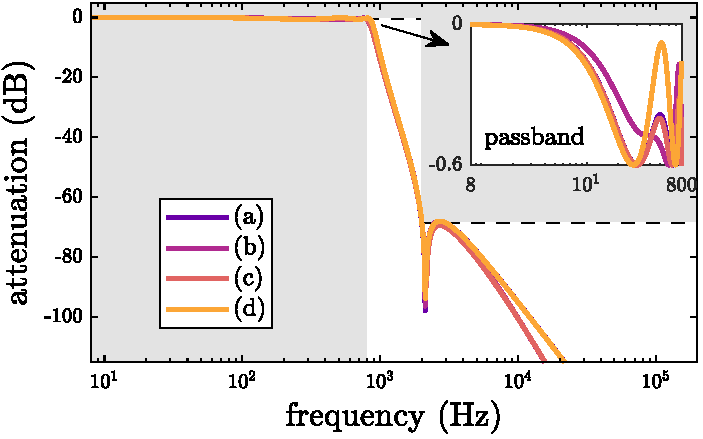
\includegraphics[width=0.5\textwidth]{../ch6/figures/reduced/r_lpf3_magnitude}
\caption{\label{fig:lpf3_magnitude}}
\end{subfigure}%

\caption[Select feasible, minimum complexity circuits and attenuation responses for \nameref{sec:ch6:lpf} task \#3.]{Select feasible, minimum complexity circuits and attenuation responses for \nameref{sec:ch6:lpf} task \#3 (units are mH and nF).\label{fig:lpf3}}

\end{figure}

The next task had slightly more stringent $K_p$ and $K_s$ limits, but the transition region was slightly larger.
Furthermore, the variables bounds are the tightest of the four tasks.
Only 197 topologies were found to be feasible, which is less than with task \#2. 
In this task, six components was the minimum number required, and four of the ten minimum complexity topologies are shown in Figs.~\ref{fig:lpf3_circuita}--\ref{fig:lpf3_circuitd} (all ten circuits are shown in Fig.~\ref{fig:app2:lpf3}). The minimum inductor topology is illustrated in Fig.~\ref{fig:lpf3_circuita}. 
Their attenuation responses are shown in Fig.~\ref{fig:lpf3_magnitude}, and all responses are within the specifications.
The circuit in Fig.~\ref{fig:lpf3_circuitc} is the same topology found in Ref.~\cite{Das2007a}, which is another case of an evolutionary approach arriving at a minimum complexity circuit.

% study 4
\begin{figure}
\centering
\begin{subfigure}[t]{0.3\textwidth}
\centering
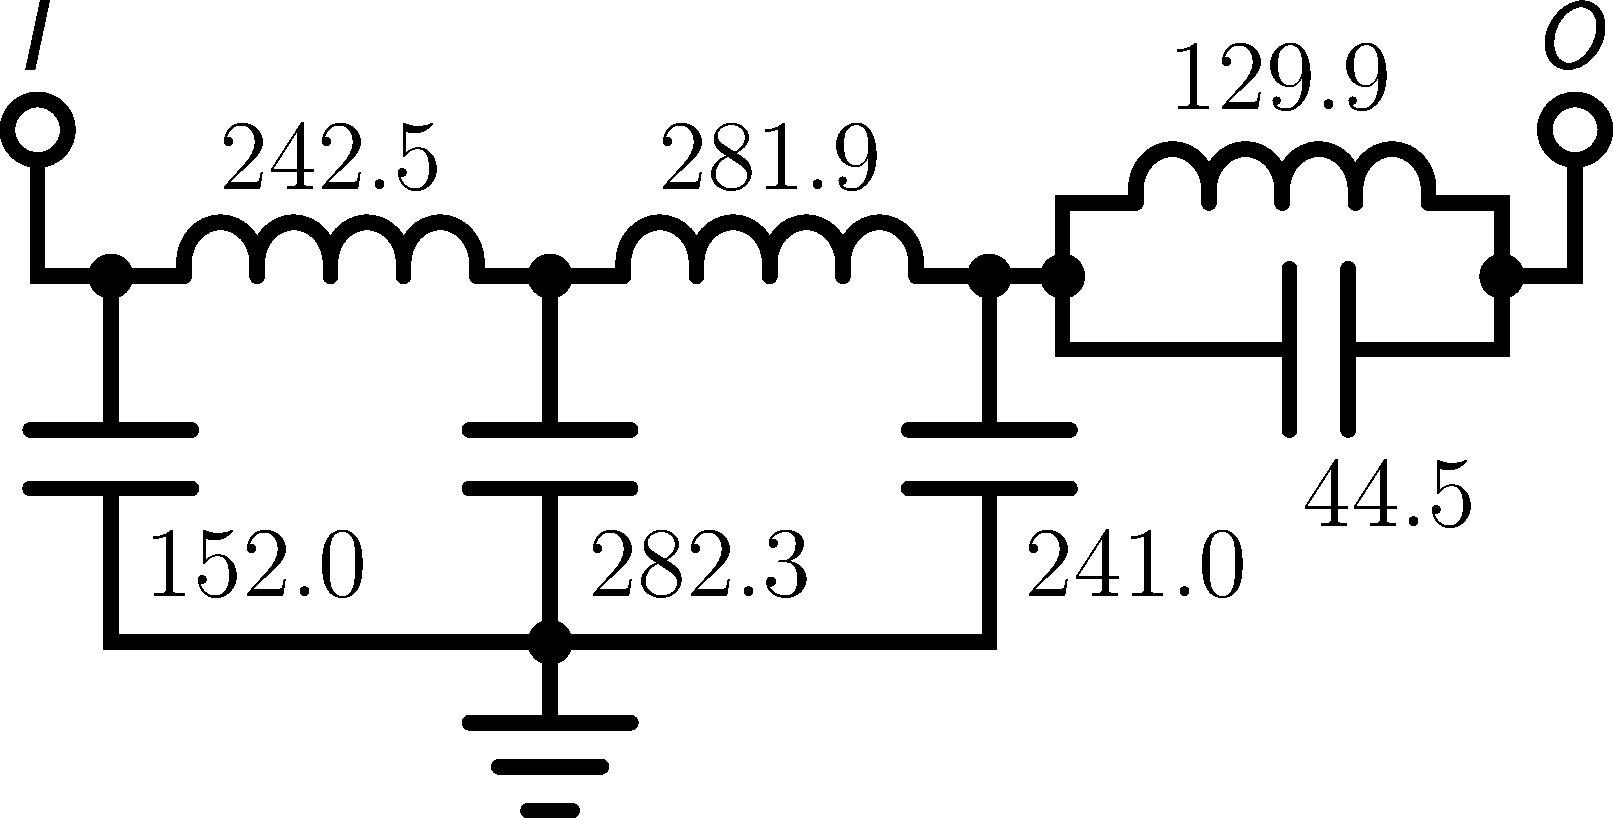
\includegraphics[scale = 0.14]{../ch6/figures/lpf4_circuit1}
\caption{$\{0.0875, 63.08\}$.\label{fig:lpf4_circuita}}
\end{subfigure}%
\begin{subfigure}[t]{0.3\textwidth}
\centering
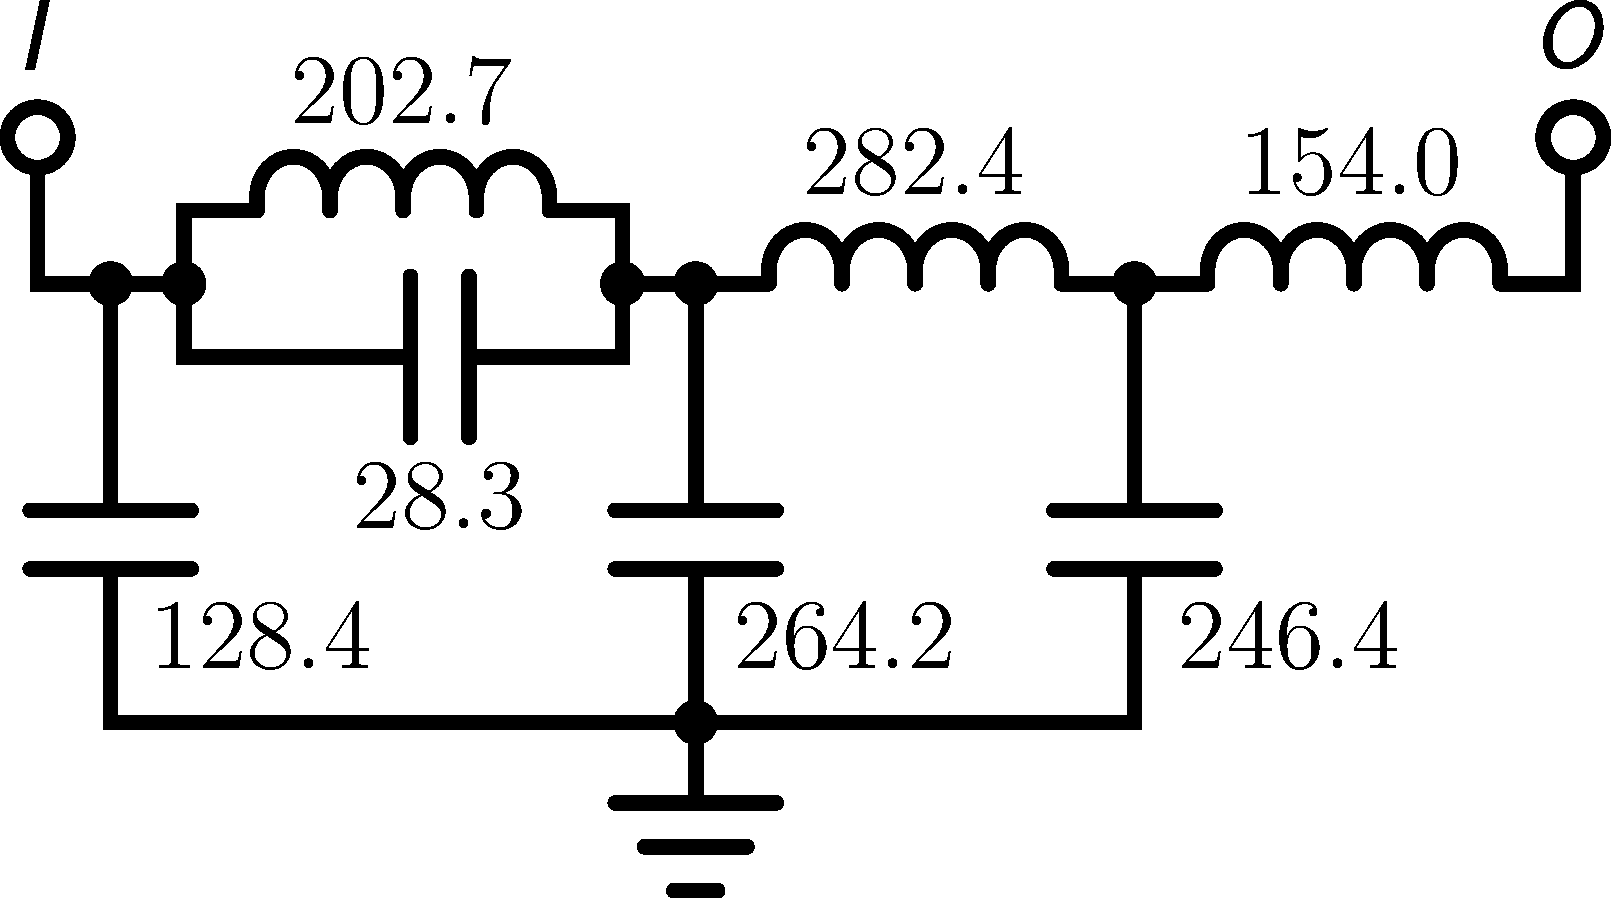
\includegraphics[scale = 0.14]{../ch6/figures/lpf4_circuit2}
\caption{$\{0.1222, 62.92\}$.\label{fig:lpf4_circuitb}}
\end{subfigure}%

\caption[Top two closest to be feasible circuits for \nameref{sec:ch6:lpf} task \#4.]{Top two closest to be feasible circuits for \nameref{sec:ch6:lpf} task \#4 and realized gains $\{K_p,K_s\}$ with respect to $f_p=1000$ Hz and $f_s=2000$ Hz (units are mH and nF).\label{fig:lpf4}}

\end{figure}

Task \#4 had the toughest specifications, primarily due to $K_p = 0.01$.
Since the requirements were equal to or more stringent than those in task \#2, only the 280 feasible circuits from task \#2 were tested, greatly reducing the computational cost. 
None of the topologies produced a feasible circuit, so we come to the conclusion that at least eight components are needed.
In Ref.~\cite{Lohn1999a}, 21 components were needed, but in Ref.~\cite{Goh2001a}, only 12 components.
Therefore, we now know that between 8 and 12 components are required to produce a feasible design.

% new paragraph
The top two circuits (in terms of performance) are shown in Fig.~\ref{fig:lpf4}.
As expected, they both include seven components, which was the limit.
The topologies are similar to minimum complexity topologies found in the previous tasks. 
Fig.~\ref{fig:lpf4_circuita} is similar to Fig.~\ref{fig:lpf3_circuitb}, and Fig.~\ref{fig:lpf4_circuitb} is similar to Fig.~\ref{fig:lpf3_circuita}.
For the best circuit, the gains $\{K_p,K_s\}$ were found to be $\{0.0875, 63.08\}$, which are a substantial improvement compared to task \#2, but still do not meet this task's stringent specifications.